\documentclass[11pt, a4paper, twoside]{article}

\input{../figuresLaTeX/introUNLaM}


\begin{document}
\begin{center}
  % \textsc{\large Mecánica general}\\
  \textsc{\large Simulation | Numerical solutions for the Euler-Lagrange equation}
\end{center}

\noindent
In the following exercises, you will solve numerically the Euler-Lagrange equation for each generalized coordinate. Plotting these solutions, using the given initial conditions and within the given time ranges, you will be simulating the dynamics of these systems.\\
Use \(|\vec{g}| = \SI{9.81}{\metre\per\second\squared}\) for the magnitude of the acceleration due to gravity.\\
Exercises marked with (*) have extra difficulty, don't hesitate to ask for help.


\begin{enumerate}


\item 
\begin{minipage}[t][2.5cm]{0.7\textwidth}
\textbf{Atwood machine}\\
Time from \(t = \SI{0}{\second}\) to \(t = \SI{10}{\second}\).
Parameters and initial conditions:\\
\(\ell_\mathrm{rope} > \SI{150}{\metre}\), 
\(R = \SI{0.5}{\metre}\), \\ 
\(m_1 = \SI{8}{\kilo\gram}\), 
\(m_2 = \SI{1}{\kilo\gram}\), 
\(m_p = \SI{4}{\kilo\gram}\), \\
\(x_1(t=0) = \SI{25}{\metre}\), 
\(\dot{x}_1(t=0) = -\SI{10}{\metre\per\second}\).
\end{minipage}
\begin{minipage}[c][2cm][t]{0.3\textwidth}
	%\hspace{0.5cm}
	%\includegraphics[width=0.6\textwidth]{marion_fig2_1a}
	\begin{tikzpicture}
	
	% pulley at 0,0
	\def \pulleyRadius {1.0};
	\coordinate (pulleyCentre) at (0,0);
	\fill [inner color = white, outer color = gray!25, thin] (pulleyCentre) circle (\pulleyRadius) node [below = 2mm] {\(m_p\)};
	\filldraw (pulleyCentre) circle (1 mm);

	% dashed lines from 0.1 at each side of the circle
	\def \deltax {1.0};
	\draw [dashed] (0.2,0) -- ({\pulleyRadius + \deltax},0);
	\draw [dashed] (-0.2,0) -- ({-\pulleyRadius - \deltax},0);
	\node at ({\pulleyRadius / 2}, 0) [above] {\(R\)};

	% weight m_1
	\def \boxwidth {\pulleyRadius/ 2.5};
	\def \boxAheight {-1.5};
	\shade [ball color=black!80] (-\pulleyRadius, \boxAheight) circle (\boxwidth) node {\color{white} $m_1$};
	
	% lower pulley
	\def \lowerPulleyHeight {-2.5};
	\shade [ball color=black!80] (\pulleyRadius, \lowerPulleyHeight) circle (\boxwidth) node {\color{white} $m_2$};
	
	% draw the line connecting the two boxes to the circle
	\draw [ultra thick] (-\pulleyRadius, \boxAheight + \boxwidth) -- (-\pulleyRadius,0);
	\draw [ultra thick] ( \pulleyRadius, \lowerPulleyHeight + \boxwidth) -- (\pulleyRadius,0); 
	\draw [ultra thick] (pulleyCentre) ++(0:\pulleyRadius) arc (0:180:\pulleyRadius);

	% draw dashed lines for y coordinates from horizontal lines to the height of middle of the boxes
	\def \pendeLeft {-\pulleyRadius - \boxwidth - 0.2};
	\def \pende {\pulleyRadius + \boxwidth + 0.2};
	\def \pendePulley {2* \pulleyRadius + 0.2};
	\draw [-Latex] (\pendeLeft, 0) -- (\pendeLeft, \boxAheight) node [midway, left] {\(x_1\)};
	\draw [-Latex] ( \pende, 0) -- ( \pende, \lowerPulleyHeight) node [midway, right] {\(x_2\)};

	% pulley angle
	\def \extra {0.5};
	\draw [-Latex] (pulleyCentre) ++(110:{\pulleyRadius + \extra / 2}) arc (110 : 160 : {\pulleyRadius + \extra / 2 }) node [midway, above] {\(\theta\)};


	% ceiling
	\def \ceilingAbove {1.5};
	\draw [line width = 1 mm] ($(pulleyCentre) + (0,\ceilingAbove)$) -- (pulleyCentre);
	\draw [ultra thick] ($(pulleyCentre) + ({- \pulleyRadius},\ceilingAbove)$)  -- ($(pulleyCentre) + (\pulleyRadius,\ceilingAbove)$);
	\fill [pattern = north east lines] ($(pulleyCentre) + ({- \pulleyRadius},\ceilingAbove)$)  rectangle ($(pulleyCentre) + (\pulleyRadius, {\ceilingAbove + 0.2 })$);


\end{tikzpicture}
\end{minipage}

\item
	a) \textbf{Ideal pendulum} [Marion ex. 7.2] \\
	b) \textbf{Pendulum with free support} [Landau \S5 ex. 2]\\ 
	c) \textbf{Double pendulum} [Landau \S5 ex. 1] 
\begin{tasks}(3)
	\task 	\begin{tikzpicture}[scale= 1.3]
  	\draw [arrows=-latex] (-1,2) -> (-1,1) node [above=15, right=2] {\(\vec{g}\)}; % g vertical
		\draw [ultra thick] (-1.5,3) -- (2,3);
		\fill [pattern = north east lines] (-1.5,3) rectangle (2,3.2); % techo
		\draw [dashed] (0,3) -- (0,-.25);	% vertical
		\draw [thick] (0,3) -- +(-60:3) node[midway,above,right=2] {\(\ell\)};	% inclinada +:relativa, -60 grados, longitud 3
		\shade [ball color=black!80] ($(0,3)+(-60:3)$) circle(0.25) node [] {\color{white} $m$};
    %\draw [arrows=-latex] (0,.4) -> (1.25,.4) node [midway, above] {\( \psi \)}; % desplazamiento horizontal
		\draw [arrows=-latex] (0,0) arc [start angle=-90, end angle=-65, radius=3] node [below=12, left=8] {\( \varphi \)};
	\end{tikzpicture}
	\task \includegraphics[height=0.24\textwidth]{figures/landauS52_fig2}
	\task \includegraphics[height=0.24\textwidth]{figures/landauS52_fig1}
\end{tasks}
Time from \(t = \SI{0}{\second}\) to \(t = \SI{10}{\second}\). Parameters and initial conditions:
\begin{enumerate}
	\item \(m = \SI{3}{\kilo\gram}\), 
				\(\ell = \SI{2}{\metre}\), 
				\(\varphi (t=0) = \frac{\pi}{4}\), \(\dot{\varphi} (t=0) = 0\).
	\item \(m_1 = \SI{3}{\kilo\gram}\), \(m_2 = \SI{1}{\kilo\gram}\),   
				\(\ell = \SI{2}{\metre}\), 
				\(x(t=0) = \SI{1}{\metre}\), \(\dot{x} (t=0) = \SI{0.5}{\metre\per\second} \),
				\(\phi (t=0) = \frac{\pi}{8}\), \(\dot{\phi} (t=0) = 0\).
	\item \(m_1 = \SI{3}{\kilo\gram}\), \(m_2 = \SI{1}{\kilo\gram}\),
				\(\ell_1 = \SI{1}{\metre}\), \(\ell_2 = \SI{1}{\metre}\),\\ 
				\(\phi_1 (t=0) = \frac{\pi}{8}\), \(\dot{\phi}_1 (t=0) = 0\), 
				\(\phi_2 (t=0) = \frac{\pi}{4}\), \(\dot{\phi}_2 (t=0) = -\frac{\pi}{16} \si{\per\second}\).
\end{enumerate}


\item 
	\begin{minipage}[t][2cm]{0.7\textwidth}
	\textbf{Pendulum of linked beads moving on rigid thin wires}\\
	Time from \(t = \SI{0}{\second}\) to \(t = \SI{10}{\second}\). Parameters and initial conditions:\\
	\(m_1 = m_2 = m = \SI{2}{\kilo\gram}\), \(l = \SI{2}{\metre}\), \(\theta(t=0) = \frac{\pi}{4}\), \(\dot{\theta}(t=0) = 0\).
	\end{minipage}
	\begin{minipage}[c][2cm][t]{0.3\textwidth}
		\hspace{0.5cm}
				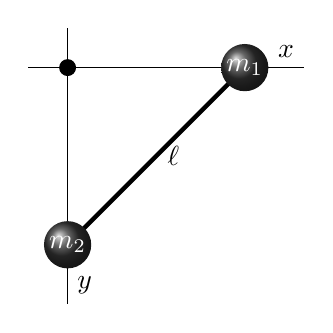
\begin{tikzpicture}


	% horizontal bar
	\def \barLength {3};
	\def \barAltitude {0};
	\def \barExtra {0.5};
	\draw [thin] (-\barExtra,\barAltitude) -- (\barLength,\barAltitude) node [above left] {\(x\)};

	% vbar
	\def \vbarHorizontal {0};
	\draw [thin] (\vbarHorizontal,\barExtra) -- (\vbarHorizontal, - \barLength) node [above right] {\(y\)};
	
	% weight centres
	\def \hbarWeightAltitude {3* \barLength / 4};
	\coordinate (hbarWeightCentre) at (\hbarWeightAltitude, \barAltitude);
	\coordinate (vbarWeightCentre) at (\vbarHorizontal, - \hbarWeightAltitude);

	% rigid bar joining weights
	\draw [ultra thick] (vbarWeightCentre) -- (hbarWeightCentre) node [midway, right] {\(\ell\)};
	

	% hbar weight
	\def \hbarWeightRadius {.3};
	\shade [ball color=black!80] (hbarWeightCentre) circle (\hbarWeightRadius) node {\color{white} $m_{1}$};

	% vbar weight
	\shade [ball color=black!80] (vbarWeightCentre) circle (\hbarWeightRadius) node {\color{white} $m_{2}$};

	% arc centred at vbarWeightCentre from 45 to 90 with radius hbarWeightRadius + barExtra/2
	%\draw [Latex-Latex] (vbarWeightCentre) ++(45:{\hbarWeightRadius + \barExtra}) arc (45:90:{\hbarWeightRadius + \barExtra}) node [midway, above right] {\(\theta\)};

	% \draw [-Latex] (vbarWeightCentre) ++(45:{\hbarWeightRadius + \barExtra / 2}) arc (0:45:{\hbarWeightRadius + \barExtra / 2 }) node [midway, right] {\(\theta\)};
	% \draw [-Latex] (vbarWeightCentre) ++(45:{\hbarWeightRadius + \barExtra / 2}) arc (0:45:{\hbarWeightRadius + \barExtra / 2 }) node [midway, right] {\(\theta\)};



	% Ring
	\def \ringRadius {0.1};
	\filldraw (0,0) circle (\ringRadius);	
	
\end{tikzpicture}
  	%  \includegraphics[width=0.6\textwidth]{figures/fcen1-004}
	\end{minipage}

	\newpage

\item
\begin{minipage}[t][2cm]{0.65\textwidth}
(*) \textbf{Compound Atwood machine} [Marion ex. 7.8]\\
	Time from \(t = \SI{0}{\second}\) to \(t = \SI{5}{\second}\). Parameters and initial conditions:\\
\(\ell_\text{top} = \SI{15}{\metre}\), 
\(R_{\text{top pulley}} = \SI{0.5}{\metre}\), 
\(\ell_\text{bottom} = \SI{15}{\metre}\), 
\(R_{\text{bottom pulley}} = \SI{0.5}{\metre}\),\\ 
\(m_1 = \SI{1}{\kilo\gram}\),
\(m_2 = \SI{2}{\kilo\gram}\),
\(m_3 = \SI{3}{\kilo\gram}\),
\(M_{\text{top pulley}} = \SI{4}{\kilo\gram}\),
\(M_{\text{bottom pulley}} = \SI{4}{\kilo\gram}\),\\
\(y(t=0) = \SI{1}{\metre}\), \(\dot{y}_1(t=0) = 0\),
\(y_2(t=0) = \SI{2}{\metre}\), \(\dot{y}_2(t=0) = 0\)
\end{minipage}
\begin{minipage}[c][3cm][t]{0.3\textwidth}
		\begin{tikzpicture}
	
	% upper pulley
	\def \pulleyRadius {1.0};
	\coordinate (pulleyCentre) at (0,0);
	\fill [inner color = white, outer color = gray!25, thin] (pulleyCentre) circle (\pulleyRadius) node [below = 2 mm] {\(m_p\)};
	\filldraw (pulleyCentre) circle (1 mm);

	%% lower pulley dimensions
	\def \extra {0.4};
	\draw [-Latex] (pulleyCentre) ++(110:{\pulleyRadius + \extra / 2}) arc (110 : 160 : {\pulleyRadius + \extra / 2 }) node [midway, above] {\(\theta_1\)};
	
	
	% dashed lines from 0.1 at each side of the circle
	\def \deltax {1.0};
	\draw [dashed] (0.2,0) -- ({\pulleyRadius + 2* \deltax},0);
	\draw [dashed] (-0.2,0) -- ({-\pulleyRadius - \deltax},0);
	\node at ({\pulleyRadius / 2}, 0) [above] {\(R\)};

	% weight m_1
	\def \boxwidth {\pulleyRadius/ 2.5};
	\def \boxAheight {-1.5};
	\shade [ball color=black!80] (-\pulleyRadius, \boxAheight) circle (\boxwidth) node {\color{white} $m_1$};
	
	% lower pulley
	\def \lowerPulleyHeight {-2.5};
	\coordinate (lowerPulleyCentre) at (\pulleyRadius,\lowerPulleyHeight);
	\fill [inner color = white, outer color = gray!25, thin] (lowerPulleyCentre) circle (\pulleyRadius) node [below = 2mm] {\(m_p\)};
	% \shade [ball color=black!80] (\pulleyRadius, \lowerPulleyHeight) circle (\boxwidth) node {\color{white} $m_2$};
	\filldraw (lowerPulleyCentre) circle (1 mm);
	\node at ($(lowerPulleyCentre) + ({\pulleyRadius / 2}, 0) $) [above] {\(R\)};
	
	%% lower pulley dimensions
	\draw [-Latex] (lowerPulleyCentre) ++(110:{\pulleyRadius + \extra / 2}) arc (110 : 160 : {\pulleyRadius + \extra / 2 }) node [midway, above] {\(\theta_2\)};
	
	% rope 1
	\draw [ultra thick] (-\pulleyRadius, \boxAheight + \boxwidth) -- (-\pulleyRadius,0);
	\draw [ultra thick] ( \pulleyRadius, \lowerPulleyHeight) -- (\pulleyRadius,0); 
	\draw [ultra thick] (pulleyCentre) ++(0:\pulleyRadius) arc (0:180:\pulleyRadius) node [above left] {\(\ell_1\)};


	% rope 2
	\draw [ultra thick] (lowerPulleyCentre) ++(0:\pulleyRadius) arc (0:180:\pulleyRadius) node [above left] {\(\ell_2\)};
	\def \belowPulley3 {-1.5};
	\coordinate (weight3) at ($(lowerPulleyCentre) + ( \pulleyRadius , \belowPulley3 )$);  
	\draw [ultra thick] ($(lowerPulleyCentre) + (\pulleyRadius , 0) $) -- (weight3);
	
	\def \belowPulleyHeight2 {-2.0};
	\coordinate (weight2) at ($(lowerPulleyCentre) + ( -\pulleyRadius , \belowPulleyHeight2 )$);  
	\draw [ultra thick] ($(lowerPulleyCentre) + (-\pulleyRadius , 0) $) -- (weight2);

	% weight m_3
	\shade [ball color=black!80] (weight3) circle (\boxwidth) node {\color{white} $m_3$};

	% weight m_2
	\shade [ball color=black!80] (weight2) circle (\boxwidth) node {\color{white} $m_2$};


	% upper puley dimensions
	\def \pendeLeft {-\pulleyRadius - \boxwidth - 0.2};
	\def \pende {\pulleyRadius + \boxwidth + 0.2};
	\def \pendePulley {2* \pulleyRadius + 0.2};
	\draw [-Latex] (\pendeLeft, 0) -- (\pendeLeft, \boxAheight) node [midway, left] {\(y_1\)};
	\draw [-Latex] ( \pendePulley, 0) -- ( \pendePulley, \lowerPulleyHeight) node [midway, right] {\(y_p\)};


	% lower pulley dimensions
	\draw [-Latex] ($(lowerPulleyCentre) + (\pendeLeft, 0) $) -- ($(lowerPulleyCentre) + (\pendeLeft, \belowPulleyHeight2 ) $) node [midway, left] {\(y_2\)};
	\draw [-Latex] ($(lowerPulleyCentre) + (\pende, 0) $) -- ($(lowerPulleyCentre) + (\pende, \belowPulley3 ) $) node [midway, right] {\(y_3\)};

	
	% lower pulley dashed lines
	\draw [dashed] ($ (lowerPulleyCentre) + (-0.2,0) $) -- ($ (lowerPulleyCentre) + ({-\pulleyRadius - \deltax},0) $);
	\draw [dashed] ($ (lowerPulleyCentre) + (0.2,0)$) -- ($(lowerPulleyCentre) + ({\pulleyRadius + \deltax},0) $);

	% ceiling
	\def \ceilingAbove {1.5};
	\draw [line width = 1 mm] ($(pulleyCentre) + (0,\ceilingAbove)$) -- (pulleyCentre);
	\draw [ultra thick] ($(pulleyCentre) + ({- \pulleyRadius},\ceilingAbove)$)  -- ($(pulleyCentre) + (\pulleyRadius,\ceilingAbove)$);
	\fill [pattern = north east lines] ($(pulleyCentre) + ({- \pulleyRadius},\ceilingAbove)$)  rectangle ($(pulleyCentre) + (\pulleyRadius, {\ceilingAbove + 0.2 })$);


\end{tikzpicture}
	% \includegraphics[width=\textwidth]{figures/marion_fig7_6}
\end{minipage}

\end{enumerate}
\end{document}
